\chapter{Materiais e Métodos}

Neste capítulo são descritos os procedimentos e materiais adotados no trabalho. Inicialmente, tem-se uma breve caracterização dos projetos selecionados nas organizações citadas na seção 3.4 inerente ao capítulo sobre metodologia. Posteriormente, são apontadas as atividades executadas neste estudo de acordo com o procedimento técnico pesquisa-ação.

\section{Projetos selecionados na CGDF}

Pelo fato de o presente trabalho propor um \textit{framework} que reúne as práticas complementares e fundamentais da verificação de \textit{software} (testes e inspeções), bem como conceitos da VBSE, procurou-se selecionar produtos que possuem impacto significativo na missão da CGDF e que não possuíam tais práticas sendo utilizadas no seu processo de desenvolvimento.

\subsection{Portal da Transparência do Distrito Federal}

O primeiro produto selecionado foi o Portal da Transparência do Distrito Federal (www.transparencia.df.gov.br). Esta é uma ferramenta de participação da sociedade no controle das ações do Governo. Dentre as informações disponibilizadas pelo portal, destacam-se informações sobre a contabilidade do Governo do Distrito Federal, tais como: instrumentos de planejamento, receitas públicas arrecadadas pelo Governo, despesas públicas realizadas pelo Estado, licitações dos órgãos do Governo do Distrito Federal e remuneração dos servidores.

O Portal da Transparência do Distrito Federal já se encontra em sua terceira versão. De acordo com a CGDF, a reformulação do Portal, culminando em sua terceira versão, fez com que os acessos aumentassem em cerca de 34\% em dezembro de 2016 e janeiro de 2017 em relação ao mesmo período no ano passado. A quantidade de usuários únicos no site, nesse intervalo, passou de 174.232 para 234.653 de acordo com o último levantamento.

A terceira versão do Portal foi concebida de forma a facilitar a navegação do usuário, bem como a compreensão dos dados disponibilizados. Adicionalmente, procurou-se desenvolver uma solução escalável, de forma que os dados pudessem ser utilizados por outros sistemas.

Desde o início da concepção arquitetural da terceira versão do Portal foram adotadas tecnologias modernas no âmbito do desenvolvimento de aplicações \textit{web}. Basicamente, adotou-se o \textit{framework AngularJS} para elaboração da aplicação cliente e o \textit{Spring Framework}, desenvolvido em linguagem Java, para construção da API \textit{REST (Representational State Transfer)} que é utilizada como \textit{backend}. A seguir, tem-se uma figura que exibe a página inicial do Portal e outra que exibe um esquema da arquitetura do Portal.

\begin{figure}[h]
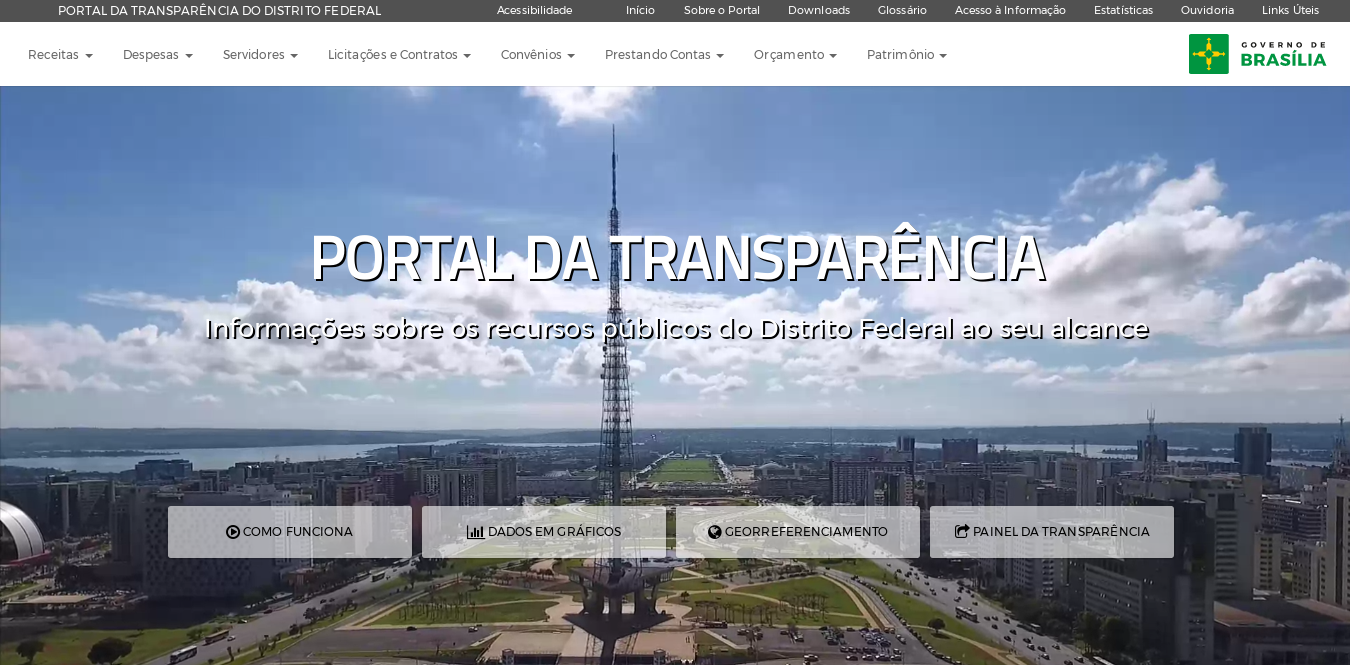
\includegraphics[width=\textwidth]{figuras/portalTransparencia.png}
\caption{Página inicial - Portal da Transparência do Distrito Federal}
\end{figure}

\begin{figure}[h]
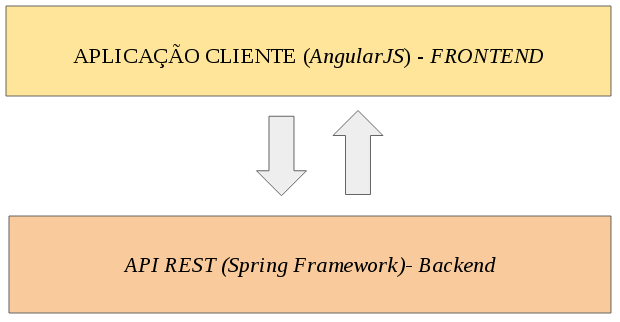
\includegraphics[width=\textwidth]{figuras/arquiteturaPortal.png}
\caption{Esquema Arquitetural - Portal da Transparência do Distrito Federal}
\end{figure}

O Portal passa por constantes evoluções. Todos os dias dados são atualizados e novas funcionalidades são incorporadas em uma periodicidade de 3 semanas, tempo de duração de uma \textit{sprint} no processo de desenvolvimento da COTEC. Assim, percebeu-se a importância de utilizar concisamente práticas da verificação de \textit{software} para melhorar a qualidade do Portal.

\subsection{Sistema de Ouvidoria do Distrito Federal}

O segundo produto selecionado foi o Sistema de Ouvidoria do Distrito Federal (www.ouv.df.gov.br). A Ouvidoria é um espaço que organiza a comunicação entre o cidadão e o governo, favorecendo a participação popular, a transparência e o aperfeiçoamento da prestação dos serviços públicos.

Como parte da estrutura da CGDF, existe a Subcontroladoria denominada Ouvidoria-Geral do DF. Esta é responsável pela coordenação dos trabalhos das Ouvidorias Especializadas - localizadas em cada órgão do Governo do Distrito Federal.

O sistema de ouvidoria também passou por uma reformulação, sendo que já se encontra em sua segunda versão. Dentre as melhorias realizadas na navegação, foram incluídas novas funcionalidades que fornecem maior transparência ao cidadão durante o atendimento de sua manifestação.

Assim como no Portal da Transparência, durante a concepção arquitetural da segunda versão do sistema de ouvidoria foram adotadas tecnologias modernas para o desenvolvimento. A camada de apresentação também utiliza o \textit{framework AngularJS} e a camada \textit{backend} foi construída utlizando a linguagem \textit{CSharp} seguindo as diretrizes do estilo arquitetural MVC (\textit{Model, View, Controller}) e também, do estilo de desenvolvimento DDD (\textit{Domain Driven Development}).

Embora tenham sido feitas boas escolhas quanto às tecnologias e arquitetura, o sistema de ouvidoria também necessita de um controle de qualidade mais rigoroso, visto que assim como o Portal, também passa por constantes evoluções. A figura a seguir exibe a página inicial do Sistema de Ouvidoria do Distrito Federal.

\begin{figure}[h]
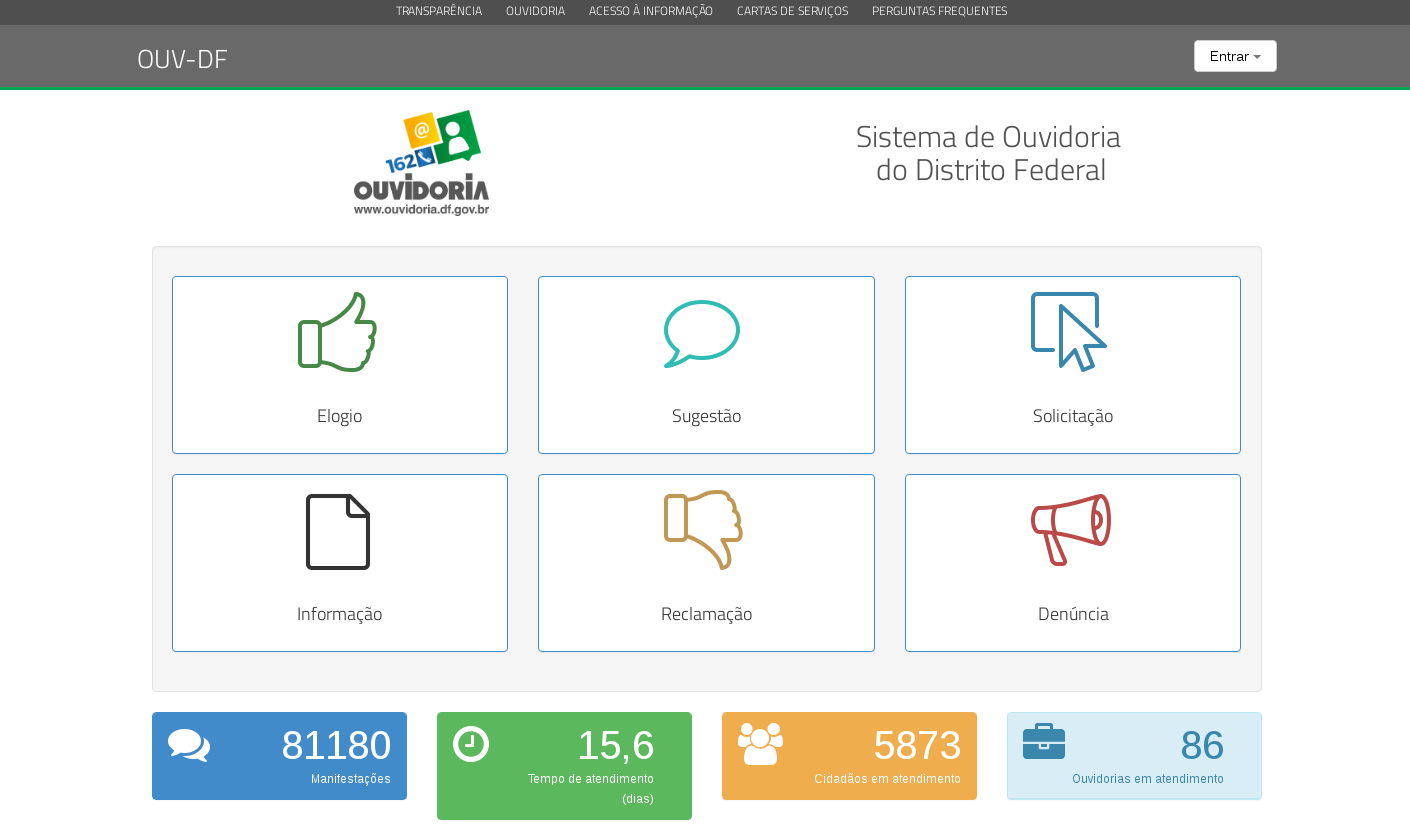
\includegraphics[width=\textwidth]{figuras/sistemaOuvidoria.png}
\caption{Página inicial - Sistema de Ouvidoria do Distrito Federal}
\end{figure}

\section{Projeto selecionado no Laboratório Fábrica de \textit{Software}}

\subsection{Aplicação de Perícia Médica}

TO DO